\documentclass[a4paper,11pt]{article}

\usepackage[french]{babel}
\usepackage[T1]{fontenc}
\usepackage[utf8]{inputenc}
\usepackage{graphicx}
\usepackage{listings}
\usepackage{color}
%\usepackage{fullpage}

\begin{document}

\title{\textbf{Compte rendu du TP \no 1 d'imagerie 3D}\\Imagerie médicale 3D}
\author{Thibaut Castanié\\\textit{Master IMAGINA}}
\date{\today}

\maketitle
\thispagestyle{empty}

\newpage 
\section{Découverte des images proposées}
Dans un premier temps, les images proposées on été ouvertes avec Fiji afin de visualiser les différentes couches d'images. Un plugin de rendu 3D permet de les superposer avec un effet de transparence, afin d'obtenir une représentation 3D de l'objet.

\begin{center}
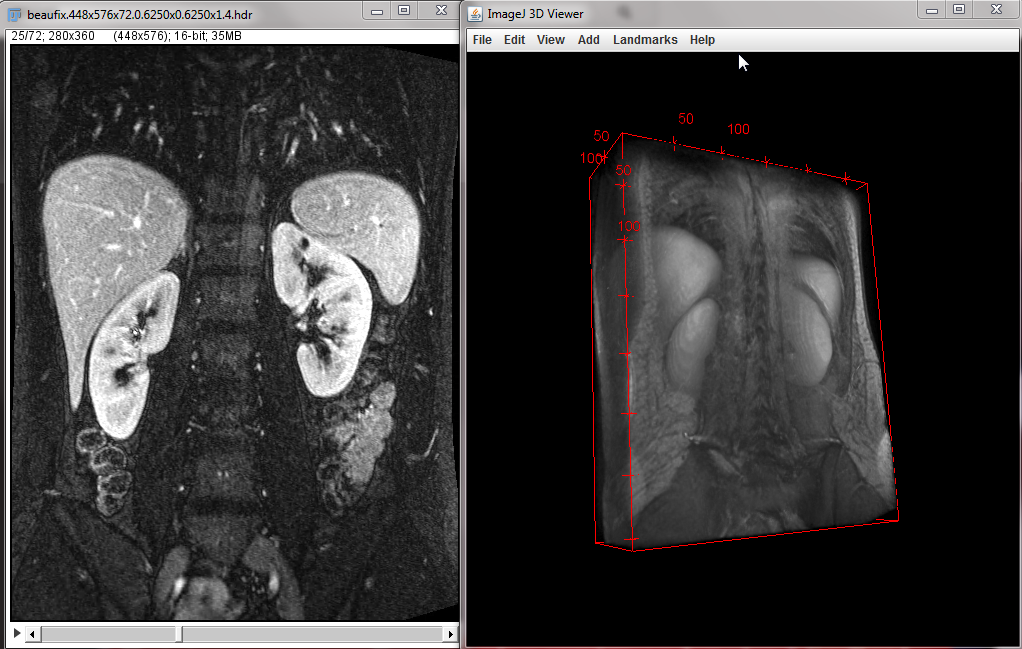
\includegraphics[scale=0.4]{beaufix.png}\\
\textit{beaufix.img représentant l'intérieur du ventre humain}
\end{center}

\begin{center}
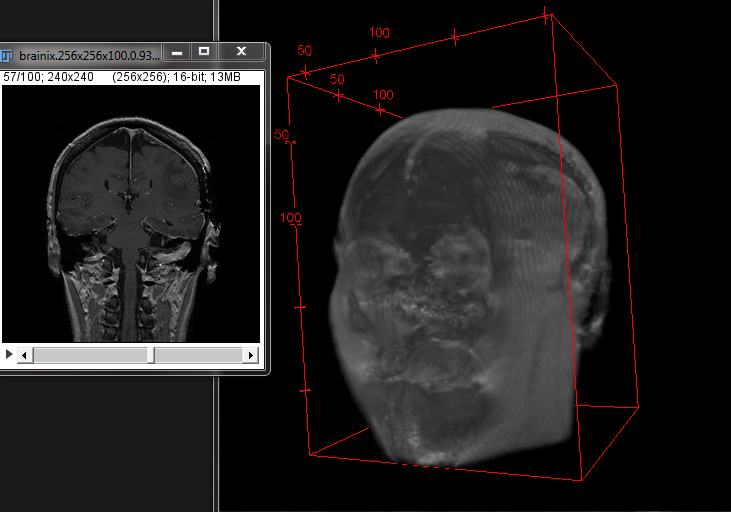
\includegraphics[scale=0.4]{brainix.png}\\
\textit{brainix.img représentant la tête d'un homme}
\end{center}

\begin{center}
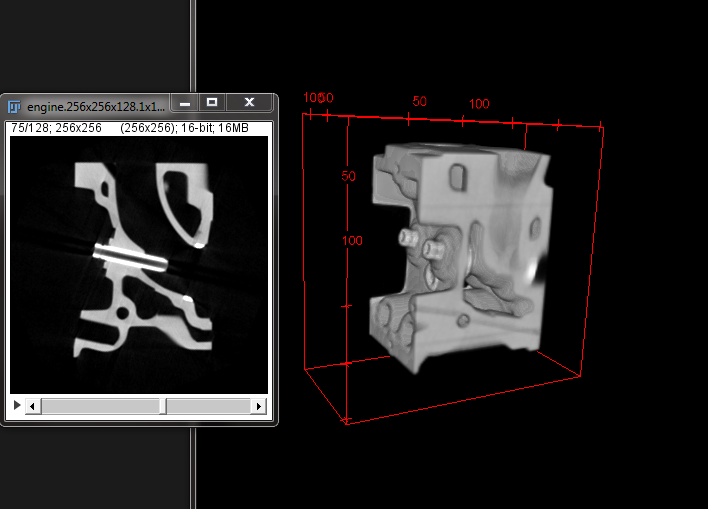
\includegraphics[scale=0.4]{engine.png}\\
\textit{engine.img représentant un moteur de voiture}
\end{center}

\begin{center}
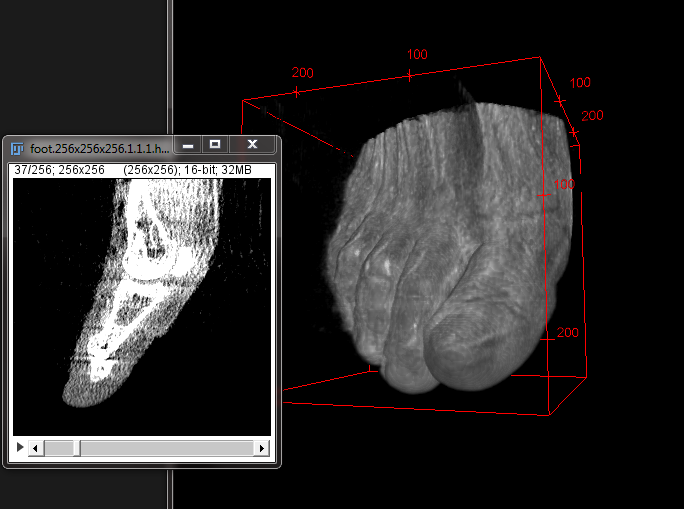
\includegraphics[scale=0.4]{footix.png}\\
\textit{foot.img représentant un pied humain}
\end{center}

\begin{center}
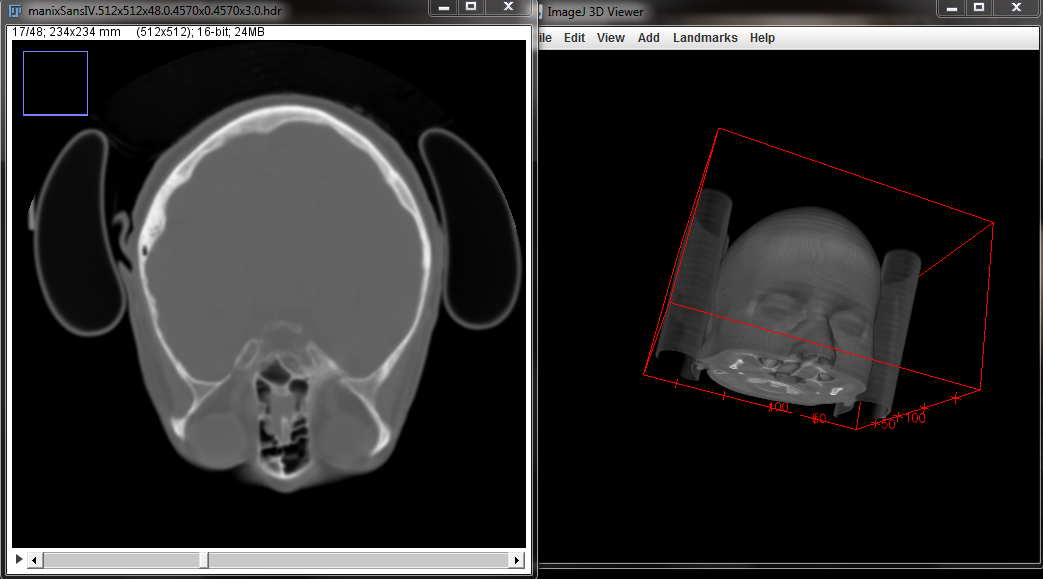
\includegraphics[scale=0.4]{manix.png}\\
\textit{manix.img représentant le cerveau d'un homme}
\end{center}

\newpage 
\section{Programme de lecture}
Afin de pouvoir manipuler les images, il a fallu créer un programme permettant de lire directement le fichier contenant les images. Celui-ci est composé d'une suite de valeur codant le niveau de gris du voxel concerné. Cette valeur est composée de deux \texttt{unsigned short} de deux bits chacun. Les valeurs sont classées de façon à lire une image après l'autre en fonction de l'axe Z de profondeur. 
\paragraph{} Faut-il écrire E6 ou 6E ? La réponse à cette question varie en fonction du logiciel utilisé lors de la capture des images ou du rendu de celles-ci. Dans notre cas, il a fallu inverser la position des \texttt{short} afin d'avoir des valeurs cohérentes.
\paragraph{} Après implémentation de l'algorithme de lecture, une série de tests a été effectuée pour vérifier la justesse du programme. Les données suivantes on étés obtenues : 
\begin{itemize}
\item  beaufix : max=334, I(200,200,20)=14
\item  branix : max=1715, I(200,200,20)=4
\item  engine : max=255, I(200,200,20)=3
\item  foot : max=255, I(200,200,20)=0
\item  manix : max=2979, I(200,200,20)=1029
\end{itemize}

\paragraph{Code en annexe}

\section{Programme de Volume Rendering}
Afin d'utiliser le programme de lecture créé, un code permettant de recréer les données en entrée, mais cette fois en prenant l'axe Z de hauteur en tant qu'axe de profondeur.
\paragraph{} Il est possible d'effectuer diverses actions sur ces données. Par exemple, le calcul de la moyenne des couches permet d'obtenir un visuel en deux dimensions qui donne une bonne idée de l'objet. En utilisant le module de rendu 3D de Fiji, on peut aussi obtenir une bonne représentation en trois dimensions de l'objet, navigable en temps réel.

\begin{center}
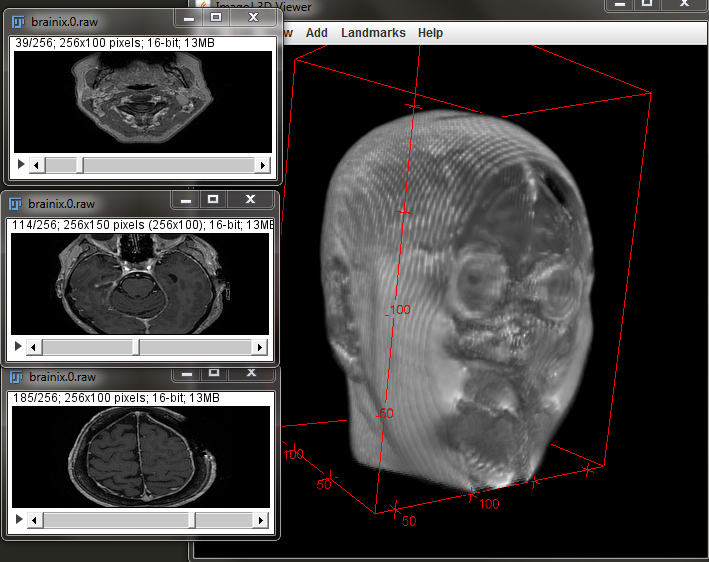
\includegraphics[scale=0.6]{brainixFait.png}\\
\textit{Visualisation de brainix, après redimensionnement du voxel en Z à 1,5}
\end{center}

\begin{center}
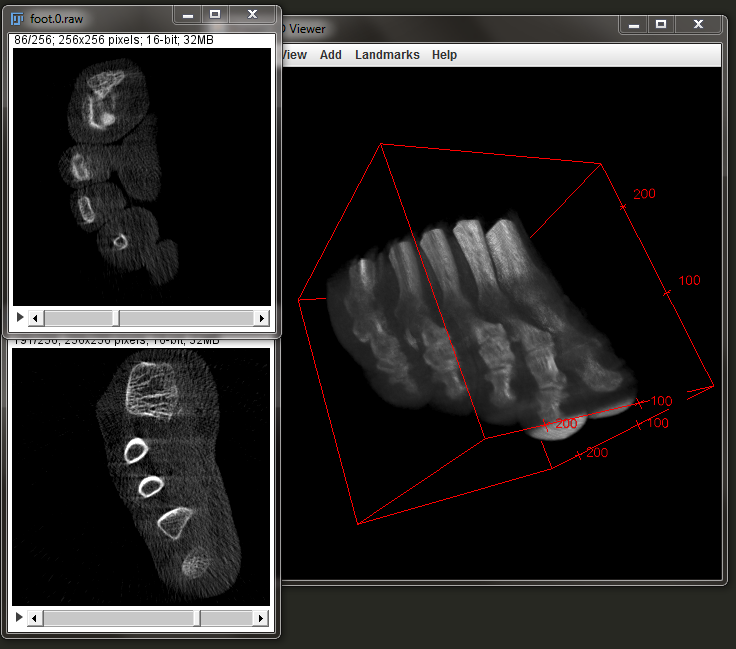
\includegraphics[scale=0.6]{footixFait.png}\\
\textit{Visualisation de foot}
\end{center}

\newpage 
\section{Qu'est ce que whatisit ?}
En effectuant la moyenne des valeurs des pixels, sur chaque couche, en fonction de l'axe Z de profondeur, on obtient une image représentant une petite écrevisse de rivière.
\begin{center}
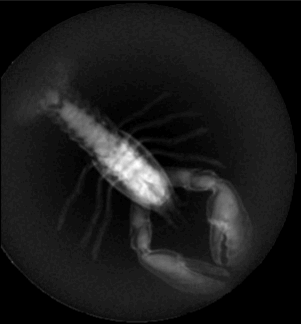
\includegraphics[scale=0.7]{ecrevisse.png}\\
\textit{Image obtenue après moyenne sur l'axe Z}
\end{center}
\begin{center}
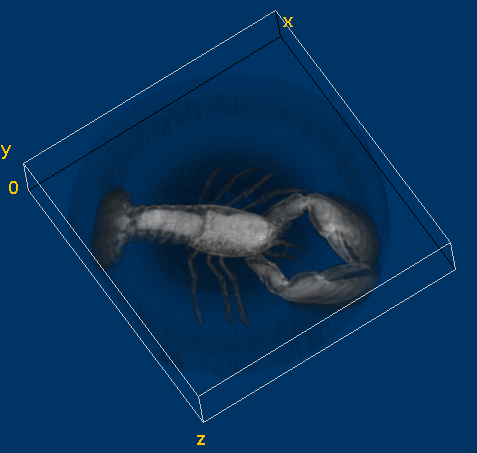
\includegraphics[scale=0.5]{ecrevisse3Dfiji.png}\\
\textit{Images obtenues visualisées en trois dimensions avec Fiji}
\end{center}


\newpage 
\section*{Annexe - Code}

\lstset{language=C++,
                basicstyle=\ttfamily,
                breaklines=true,
                keywordstyle=\color{blue}\ttfamily,
                stringstyle=\color{red}\ttfamily,
                commentstyle=\color{green}\ttfamily,
                morecomment=[l][\color{magenta}]{\#}
}

\begin{lstlisting}
#include <iostream>
#include <stdio.h>
#include <cstdlib>
#include <math.h>
#include <string> 
using namespace std;
int tailleX = 301;
int tailleY = 324;
int tailleZ = 56;
unsigned short * buffer;

int getValue(unsigned short * buffer,int x, int y, int z){
    int num = z*(tailleX*tailleY)+(y*tailleX)+x;
    int oct1 = buffer[num]%256;
    int oct2 = buffer[num]/256;
    int valPixel = oct1*256+oct2;
    return valPixel;
}

int main(int argc, char const *argv[]){
    long taille;
    size_t result;
    FILE * imgFile;
    FILE * stockFile;
    short valeurPixel = 0;
    short max = 0;
    short octet1;
    short octet2;
    //imgFile = fopen ("./BEAUFIX/beaufix.448x576x72.0.6250x0.6250x1.4.img","rb");
    //imgFile = fopen ("./BRAINIX/brainix.256x256x100.0.9375x0.9375x1.5.img","rb");
    //imgFile = fopen ("./engine/engine.256x256x128.1x1x1.img","rb");
    //imgFile = fopen ("./FOOT/foot.256x256x256.1.1.1.img","rb");
    //imgFile = fopen ("./MANIX/manixSansIV.512x512x48.0.4570x0.4570x3.0.img","rb");
    imgFile = fopen ("./WHATISIT/whatisit.301x324x56.1.1.1.4.img","rb");
    if (imgFile!=NULL){
        fseek (imgFile , 0 , SEEK_END);
        taille = ftell (imgFile);
        rewind (imgFile);
        unsigned short *buffer = new unsigned short[taille];
        result = fread (buffer,2,taille,imgFile);
        cout << result << endl;
        if (result == taille/2) {
            for (int i = 0; i < result; i++){
                octet1 = buffer[i]%256;
                octet2 = buffer[i]/256;
                int valeurPixel = octet1*256+octet2;
                if (valeurPixel > max){
                    max = valeurPixel;
                }
            }
            cout << "Max :\t" << max << endl; // valeur maximum
        }
        int retour = getValue(buffer,200,200,20);
        cout << retour << endl;
        stockFile = fopen ("whatisit.0.raw","wb");
        unsigned short *render = new unsigned short[tailleX*tailleZ*tailleY];
        int cpt=0;
        for (int k = 0; k < tailleY; k++){
            for(int i = 0; i<tailleZ;i++){
                for (int j = 0; j < tailleX; j++){
                    render[cpt] = getValue(buffer,j,k,i);
                    cpt++;
                }
            }
        }
        fwrite(render,2,tailleX*tailleZ*tailleY,stockFile);
        fclose (stockFile);
        fclose (imgFile);
        free (buffer);
    }
    return 0;
}
\end{lstlisting}

\end{document}